\documentclass{article}
\usepackage[spanish]{babel}
\usepackage[numbers,sort&compress]{natbib}
\usepackage{graphicx}
\graphicspath{ {images/} }
\usepackage{subfigure}
\usepackage{url}
\usepackage{hyperref}
\usepackage{amsmath}
\usepackage[top=15mm, bottom=40mm, left=15mm, right=15mm]{geometry}
\setlength{\parskip}{2mm}
\setlength{\parindent}{0pt}
\usepackage{listings}
\usepackage{mathrsfs}


\lstdefinestyle{mystyle}{
  numbers= left}
\lstset{style=mystyle}

\author{3175}
\title{Práctica 11: Frentes de Pareto}
\date{\today}

\begin{document}

\maketitle


\section{Introducción}

Las frentes de Pareto reciben el nombre en honor a Vilfredo Pareto, quien fué quien los enunció por primera vez ya que empíricamente observó que las poblaciones se distribuían las pertenencias entre muy pocos, por ejemplo observó que el ochenta porciento de las tierras en Italia le pertenecían al veinte porciento de las personas\citep{web1}.
 
\section{Objetivo}
Analizar por medio de la simulación de polinomios y las soluciones de estos, la distribución de soluciones de pareto utilizando diferente cantidad de funciones objetivo.

\section{Metodología}

Usando de base el código proporcionado\citep{webelisa}, se genera polinomios al azar, los cuales se van a utilizar como restricciones y funciones objetivo, además como parámetros se definieron a contenerlos cinco términos, cuatro variables y un grado máximo de tres. Posteriormente se generan las soluciones iniciales que van a ser evaluadas entre sí para construir así la frente de pareto. Para la práctica se realizaron simulaciones con funciones objetivo difetentes, comenzando con dos hasta llegar a diez, realizando $60$ repeticiones para obtener una muestra significativa y generandose al principio $200$ y $500$ soluciones iniciales.
El proceso se paralelizó mediante el uso de la librería $Parallel$:

\lstinputlisting[language= R, firstline=43, lastline=77]{P11.R}

Finalmente se realizaron 2 gráficas, con $200$ y $500$ soluciones iniciales, utilizando gráficas de violín y de caja bigote para mayor facilidad visualización\citep{web2}.


\section{Resultados}
Los resultados en las figuras 1 y 2, muestran una tendencia marcada al aumento del porcentaje de soluciones no dominadas conforme se aumenta la cantidad de funciones objetivo.
Se encontró que los resultados en ambos casos presentan diferencias significativas entre los resultados obtenidos en las diferente cantidad de funciones objetivo, debido a que al realizar la prueba ANOVA el factor de Fisher fue menor a 0.05 en ambos casos.
\begin{lstlisting}
Con 200 resultados

             Df Sum Sq Mean Sq F value Pr(>F)    
Funciones     8  56.40   7.051   177.6 <2e-16 ***
Residuals   531  21.08   0.040                   
---
Con  500 resultados
             Df Sum Sq Mean Sq F value Pr(>F)    
Funciones     8  59.79   7.473   172.1 <2e-16 ***
Residuals   531  23.06   0.043 
\end{lstlisting}

\begin{figure}[!ht]
\centering
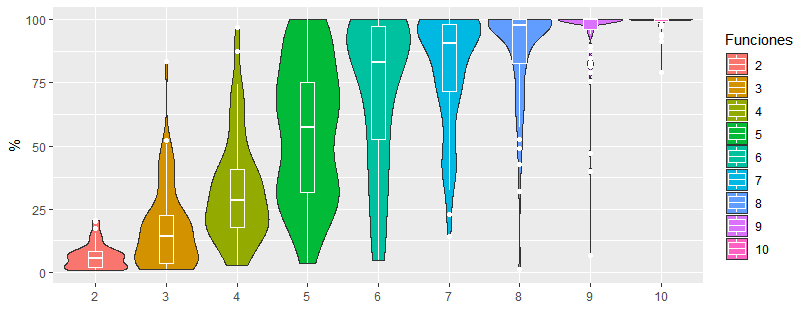
\includegraphics[width=17cm, height=8cm]{P11graf200.png}
\caption{Porcentajes de resultados dominantes encontrados con diferentes funciones objetivo generando 200 soluciones al principio}
\end{figure}

\begin{figure}[!ht]
\centering
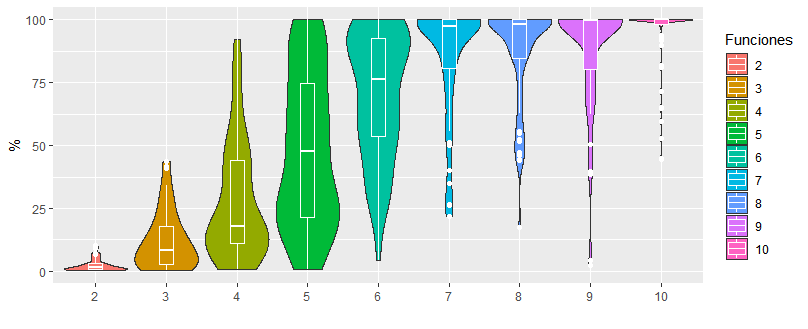
\includegraphics[width=17cm, height=8cm]{P11graf500.png}
\caption{Porcentajes de resultados dominantes encontrados con diferentes funciones objetivo generando 500 soluciones al principio}
\end{figure}


\section{Conclusiones}
Con base en los resultados obtenidos se pueden razonar que al aumentar el número de funciones objetivo aumenta el porcentaje de soluciones dominantes debido a que al buscar más objetivos las soluciones se distrubuyen entre todas éstas disminuyendo la cantidad de competencia directa entre éstas. Evidencia de ésta conclusión se puede observar ya que al aumentar el número de soluciones a $500$ en los lugares donde casi se alcanza el cien porciento se distribuye mayormente, aun que con la misma tendencia.
\bibliographystyle{plainnat}
\bibliography{biblio11}
\end{document}